\def\mySecNum{11.1}
\mySection{\mySecNum~Understanding Early Exercise}
%-------------- start slide -------------------------------%{{{ 1
\begin{frame}[fragile,t]

\begin{center}
	Options may be rationally exercised prior to expiration
\end{center}

\bigskip

\begin{itemize}
	\item[] 	By exercising, the option holder
		\bigskip
	\item[$\textcolor{magenta}{+}$] Receives the stock and thus receives dividends
		\bigskip
	\item[$\textcolor{cyan}{-}$] Pays the strike price prior to expiration (this has an interest cost)
		\bigskip
	\item[$\textcolor{cyan}{-}$] Loses the insurance implicit in the call against the possibility that the stock price will be less than the strike price at expiration
\end{itemize}
\end{frame}
%-------------- end slide -------------------------------%}}}
%-------------- start slide -------------------------------%{{{ 1
\begin{frame}[fragile,t]
\begin{myexample}
	For a call option, let $K=100$,  $r=0.05$,  $\delta=0.05$, $\sigma=0$ and the stock price today is $S=200$.
	Shall we exercise the call?
\end{myexample}
\bigskip
\pause
\begin{mysol}
	\bigskip
	\begin{itemize}
		\item[$\textcolor{magenta}{+}$] Receives the stock and thus receives dividends:
			\begin{align*}
				S \times \delta = 200\times 0.05=\textcolor{magenta}{\$ 10.00}.
			\end{align*}
		\item[$\textcolor{cyan}{-}$] Pays the strike price prior to expiration (this has an interest cost)
			\begin{align*}
				K \times r = 100\times 0.05=\textcolor{cyan}{\$ 5.00}.
			\end{align*}
		\item[$\textcolor{cyan}{-}$] Loses the insurance: $\textcolor{cyan}{\$ 0}$ because $\delta=0$.
			\bigskip
		\item[] Hence, we need to early exercise! \myEnd
	\end{itemize}
\end{mysol}
\end{frame}
%-------------- end slide -------------------------------%}}}
%-------------- start slide -------------------------------%{{{ 1
\begin{frame}[fragile]
	If \textcolor{cyan}{volatility is zero}, the value of insurance is zero. Then, it is optimal to defer exercise as long as interest savings on the strike exceed dividends lost
	\begin{align*}
		r K > \delta S
	\end{align*}
	\[\Downarrow\]
	\begin{align*}
		\text{It is optimal to exercise} \quad \Longleftrightarrow \quad S> \frac{rK}{\delta}
	\end{align*}
	\begin{itemize}
		\item[E.g.] If $r=\delta$, any in-the-money option should be exercised immediately.
		\item[] If $r=3\delta$, we exercise when the stock price is 3 times of the strike price.
	\end{itemize}
	\bigskip
	\mySeparateLine
	\bigskip
	\pause
	When \textcolor{magenta}{volatility is positive}, the implicit insurance has value that varies
	with time to expiration.
\end{frame}
%-------------- end slide -------------------------------%}}}
%-------------- start slide -------------------------------%{{{ 1
\begin{frame}[fragile,t]
	\frametitle{Early-exercise boundary \\ -- American call}
	\begin{center}
		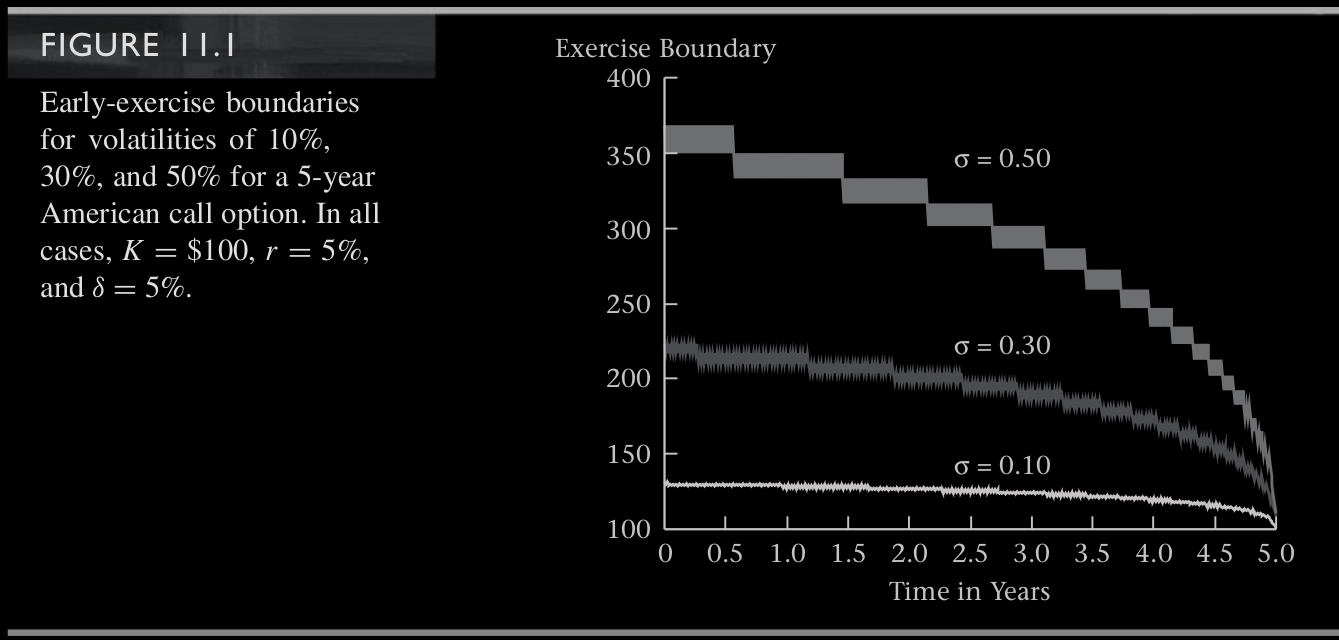
\includegraphics[scale=0.25]{figs/Figure-11-1.png}
	\end{center}
	\pause
	\begin{itemize}
		\item Curve computed using 500 binomial steps.
		\item When $\sigma=0$, the boundary should be $S=K=\$100$.
		\item The value of insurance diminishes in time.
	\end{itemize}
\end{frame}
%-------------- end slide -------------------------------%}}}
%-------------- start slide -------------------------------%{{{ 1
\begin{frame}[fragile,t]
	\frametitle{Early-exercise boundary \\ -- American put}
	\begin{center}
		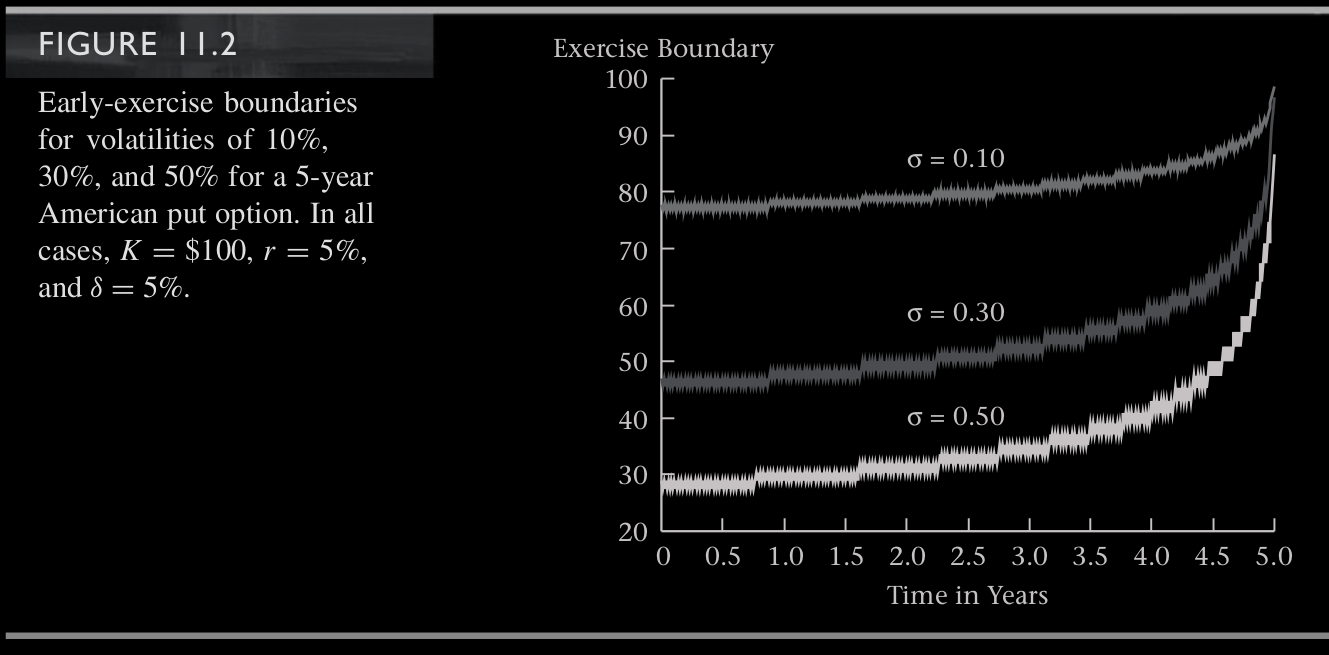
\includegraphics[scale=0.25]{figs/Figure-11-2.png}
	\end{center}
\end{frame}
%-------------- end slide -------------------------------%}}}
